%%%%%%%%%%%%%%%%%%%%%%%%%%%%%%%%%%%%%%%%%%%%%%%%%%%%%%%%%%%%%%%%%%%%%%%%%%%%%%%%
%2345678901234567890123456789012345678901234567890123456789012345678901234567890
%        1         2         3         4         5         6         7         8

\documentclass[letterpaper, 10 pt, conference]{ieeeconf}  % Comment this line out
                                                          % if you need a4paper
%\documentclass[a4paper, 10pt, conference]{ieeeconf}      % Use this line for a4
 \IEEEoverridecommandlockouts                              % This command is only
                                                          % needed if you want to
                                                             % use the \thanks
                                                          % command
\overrideIEEEmargins
% See the \addtolength command later in the file to balance the column lengths
% on the last page of the document

\usepackage[portuguese]{babel}
\usepackage[utf8]{inputenc}
\usepackage{amsmath}
\usepackage{mathtools}
\usepackage{graphicx}
\usepackage{subfigure}
\usepackage{float}
\usepackage{listings}
\usepackage[numbered, framed]{mcode}
%\usepackage[colorinlistoftodos]{todonotes}


% The following packages can be found on http:\\www.ctan.org
%\usepackage{graphics} % for pdf, bitmapped graphics files
%\usepackage{epsfig} % for postscript graphics files
%\usepackage{mathptmx} % assumes new font selection scheme installed
%\usepackage{times} % assumes new font selection scheme installed
%\usepackage{amsmath} % assumes amsmath package installed
%\usepackage{amssymb}  % assumes amsmath package installed

\title{\LARGE \bf
GPGPU aplicada ao reconhecimento ótico de caracteres utilizando técnica de N vizinho mais próximos.
}

%\author{ \parbox{3 in}{\centering Huibert Kwakernaak*
%         \thanks{*Use the $\backslash$thanks command to put information here}\\
%         Faculty of Electrical Engineering, Mathematics and Computer Science\\
%         University of Twente\\
%         7500 AE Enschede, The Netherlands\\
%         {\tt\small h.kwakernaak@autsubmit.com}}
%         \hspace*{ 0.5 in}
%         \parbox{3 in}{ \centering Pradeep Misra**
%         \thanks{**The footnote marks may be inserted manually}\\
%        Department of Electrical Engineering \\
%         Wright State University\\
%         Dayton, OH 45435, USA\\
%         {\tt\small pmisra@cs.wright.edu}}
%}

\author{David Clifte$^{1}$  Gustavo Siebra$^{2}$% <-this % stops a space
%\thanks{*This work was not supported by any organization}% <-this % stops a space
%\thanks{$^{1}$H. Kwakernaak is with Faculty of Electrical Engineering, Mathematics and Computer Science,
%        University of Twente, 7500 AE Enschede, The Netherlands
%        {\tt\small h.kwakernaak at papercept.net}}%
%\thanks{$^{2}$P. Misra is with the Department of Electrical Engineering, Wright State University,
%        Dayton, OH 45435, USA
%        {\tt\small p.misra at ieee.org}}%
}


\begin{document}



\maketitle
\thispagestyle{empty}
\pagestyle{empty}


%%%%%%%%%%%%%%%%%%%%%%%%%%%%%%%%%%%%%%%%%%%%%%%%%%%%%%%%%%%%%%%%%%%%%%%%%%%%%%%%
\begin{abstract}

Este artigo descreve o uso dos k-vizinhos mais próximos, visão computacional e paralelismo para
analisar o custo das imagens recebidas de um scanner ou outra forma de digitalização
para reconhecer o dígito manuscrito e classificá-lo de 0-9, ou indefinido, de acordo com
o valor correspondente. As principais características do sistema são: Controlar o grau
de acerto, um sistema de autoaprendizagem de fácil implementação e modularizado.

\end{abstract}


%%%%%%%%%%%%%%%%%%%%%%%%%%%%%%%%%%%%%%%%%%%%%%%%%%%%%%%%%%%%%%%%%%%%%%%%%%%%%%%%
\section{INTRODUÇÃO}

O reconhecimento ótico de caracteres (OCR) permite que uma máquina possa
reconhecer automaticamente um caractere através de um mecanismo óptico. As tentativas
da engenharia em reconhecer caracteres impressos, ou manuscritos, iniciaram antes da
Segunda Guerra Mundial, mas isso não foi possível até a década de 50, quando a associação
dos Bancos e a Indústria dos serviços financeiros criaram fundos para a pesquisa e
desenvolvimento da tecnologia [1].Diante da necessidade de uma abordagem mais simples
aos temas de visão computacional e algoritmos de inteligência computacional, ambos tem
custo computacional alto devido as rotinas necessárias para aplicações com OCR, foi
desenvolvido um sistema para diminuir o custo com o suporte de placas gráficas GPU.

Computadores podem executar muitas operações com um tempo consideravelmente
menor que os humanos poderiam fazer. Contudo, nem sempre, essa rapidez é a melhor
escolha para resolver um problema. Muitas tarefas com as quais os computadores falham
consideravelmente os humanos fazem melhor. Muitas dessas tarefas, nas quais os computadores
perdem estão relacionadas à natureza interpretativa e de multi-processamento do
cérebro. Uma maneira simples de caracterizar bem a diferença entre o computador e o
Homem seria comparar o computador, que é uma máquina serial, com o nosso cérebro,
que é altamente paralelo e possui como característica principal a capacidade de aprender
coisas [3].

O k-vizinhos mais próximos (kNN) problema de pesquisa é amplamente utilizado em domínios e aplicações, tais como a classificação, estatísticas e biologia. Neste trabalho, propomos uma implementação baseada em GPU rápida do algoritmo força bruta de busca kNN usando o CUDA

%%%%%%%%%%%%%%%%%%%%%%%%%%%%%%%%%%%%%%%%%%%%%%%%%%%%%%%%%%%%%%%%%%%%%%%%%%%%%%%%
\section{RECONHECIMENTO ÓTICO DE CARACTERES}

\subsection{Pré-Processamento}

O pré-processamento de imagens consiste na aplicação de técnicas para realce
de imagens, que visam destacar uma região dentro da imagem, permitindo a
sua visualização com mais detalhes, de modo que a imagem resultante seja mais
apropriada para uma aplicação específica do que a imagem original. Neste trabalho,
a fim de analisar a eficácia dessas transformações em imagens digitais,
foram abordadas algumas técnicas de pré-processamento como limiarização adaptativa, elemento estruturante, dilatação, erosão, detecção de componentes conexos e extração de características.\\

%%%%%%%%%%%%%%%%%%%%%%%%%%%%%%%%%%%%%%%%%%%%%%%%%%%%%%%%%%%%%%%%%%%%%%%%%%%%%%%%
\subsubsection{Limiarização Adaptativa}

A segmentação de imagens é um processo que tipicamente particiona o domínio espacial de uma imagem em subconjuntos mutuamente exclusivos, chamados regiões, onde cada região é uniforme e homogênea com respeito a algumas propriedades como tom ou textura e cujos valores diferem, em alguns aspectos e significados, das propriedades de cada região vizinha. 

A limiarização de uma imagem digital é um método que se baseia no histograma da imagem, buscando encontrar regiões bem definidas, afim de poder efetuar a divisão da imagem em objetos ou regiões. A continuidade dos níveis de cinza é a primitiva de maior valor na segmentação por região. Assim, a limiarização efetua a subdivisão da imagem em função das regiões realmente significativas contidas no seu histograma [5]. 

A limiarização global usa um limiar fixo para todos os pixels na imagem e, por esta razão, resultados realmente satisfatórios serão obtidos quando o histograma de distribuição de níveis de cinza contém cumes distintos e separados que correspondem aos objetos e ao fundo. Isto conduz a conclusão que um limiar local deve ser usado.\\

• A imagem original é dividida em sub-imagens;\\

• Um limiar é determinado independentemente para cada sub-imagem;\\

• Se um limiar não puder ser determinado para alguma sub-imagem, ele pode ser interpolado à partir dos limiares determinados nas sub-imagens vizinhas;\\

• Cada sub-imagem é então processada utilizando seu limiar local.\\

A limiarização adaptativa é uma técnica que analisa diversos aspectos da imagem para definir se determinado pixel será considerado preto ou branco. Esta técnica possui uma literatura repleta de algoritmos, desde soluções simples (que requer pouco custo computacional) ate a solução ótima de limiarização local. Os algoritmos baseiam-se em características variadas da imagem, como o formato do histograma, a entropia do histograma, atributos espaciais, entre outros. Uma definição de um limiar para técnicas adaptativas pode ser denotada
como sendo:

\begin{align}
T=T[x,y,p(x,y),f(x,y)]
\end{align}
\\Sendo f(x,y) é o nível de cinza do ponto (x,y) na imagem original, e p(x,y) é
alguma propriedade local deste ponto. Percebe-se que o limiar T não depende
apenas do nível de cinza do ponto. É necessário atenção especial ao fator p(x,y) que
é descrito como uma propriedade do ponto e que é, um dos mais importantes
componentes no cálculo do limiar para um certo ponto [MIL98]. Para que a influência
de ruído ou iluminação possa ser levada em conta, o cálculo dessa propriedade é
baseado no ambiente em que o ponto em questão está inserido. Um exemplo de
propriedade é a média dos níveis de cinza em uma vizinhança pré-estabelecida, na
qual o centro é o ponto em análise. Este método produzirá os resultados desejados.

%%%%%%%%%%%%%%%%%%%%%%%%%%%%%%%%%%%%%%%%%%%%%%%%%%%%%%%%%%%%%%%%%%%%%%%%%%%%%%%%
\subsection{Morfologia Matemática}

A morfologia matemática é a parte do processamento de imagem não-linear que tem por objetivo extrair características da imagem associadas à geometria dos objetos. Foi desenvolvida inicialmente por Georges Matheron e Jean Serra na década de 60, para imagens binárias utilizando a teoria de conjuntos. Posteriormente, ela foi estendida para imagens em tons cinza (funções) utilizando a teoria de reticulados, onde uma imagem é vista como a superfície de um relevo.\\

\subsubsection{Elemento Estruturante}

Uma transformação morfológica consiste essencialmente da comparação da imagem com outra menor, cuja geometria é conhecida, denominada elemento estruturante. Um elemento estruturante planar é um conjunto de coordenadas de pixel. Por exemplo, o elemento cruz é definido por E = \{(0,1,0);(1,1,1);(0,1,0)\}. Uma transformação morfológica requer uma operação não-linear entre a imagem e o elemento estruturante, o qual desliza sobre a imagem de forma similar à convolução discreta. Neste sentido, o elemento estruturante planar define uma relação de adjacência do tipo (p, q) $\in$ A se q - p $\in$ E. Um elemento estruturante não-planar é um par (E,V) que consiste de um conjunto de coordenadas de pixel E e um conjunto de valores V associados a cada coordenada, assim como uma imagem. Por exemplo, $ V = \{2, 1, 1, 1, 1\} $ para o caso do elemento cruz. Este tipo de elemento é usado apenas em operações com imagens em tons de cinza. Neste caso, o elemento estruturante pode ser visto como uma máscara de convolução, muito embora a operação seja outra. No caso particular, onde todos valores em V são zero, o elemento estruturante se torna planar.\\

%%%%%%%%%%%%%%%%%%%%%%%%%%%%%%%%%%%%%%%%%%%%%%%%%%%%%%%%%%%%%%%%%%%%%%%%%%%%%%%%
\subsubsection{Dilatação}

É uma transformação morfológica que combina dois conjuntos usando adição vetorial. Seu símbolo é $\oplus$. Como o nome diz, o resultado será uma imagem “engordada”. A dilatação de um conjunto A pelo conjunto B é definida por:

\begin{center}
\textbf {A $\oplus$ B = \{ c $\mid$ c = a + b , a $\in$ A , b $\in$ B \}} \\
\end{center}

Onde A representa a imagem sendo operada e B é um segundo conjunto onde é chamado elemento estrutural e sua composição define a natureza especifica da dilatação, sendo assim a dilatação expande uma imagem. Ela pode ser representada pela união A $\oplus$ B = A $\cup$ B.\\

Seja o conjunto A = \{(0,1);(1,1);(2,1);(2,2);(3,0)\} e B = \{(0,0);(0,1)\} então o resultante da dilatação é:\\

\textbf A $\oplus$ B = \{A + \{(x1 $\in$ B)\} $\cup$ A + \{(x2 $\in$ B)\}\}

\textbf A $\oplus$ B = \{(0,1);(1,1);(2,1);(3,0);(0,2);(1,2);(2,2);(2,3);(3,1)\}\\

Uma aplicação da dilatação é o preenchimento de buracos, ver Figura \ref{fig:Figura01}:

\begin{figure}[H]
\centering

\subfigure[Imagem Original]{ \includegraphics[height=3cm]{dog.jpg}}
\subfigure[Dilatação - square]{ \includegraphics[height=3cm]{dilate1.jpg}}\\
\subfigure[Dilatação - line]{ \includegraphics[height=3cm]{dilate2.jpg}}
\subfigure[Dilatação - disk]{ \includegraphics[height=3cm]{dilate3.jpg}}


\caption{Resultados da Dilatação com diferentes Elementos Estruturantes}
\label{fig:Figura01}
\end{figure}

%%%%%%%%%%%%%%%%%%%%%%%%%%%%%%%%%%%%%%%%%%%%%%%%%%%%%%%%%%%%%%%%%%%%%%%%%%%%%%%%
\subsubsection{Erosão}

A erosão basicamente encolhe uma imagem e pode ser vista como uma transformação morfológica que combina dois conjuntos usando vetores de subtração. Ela é expressa como a interseção de A e B. Assim e definido A $\ominus$ B = B $\cap$ A. A erosão da imagem A pelo elemento estrutural B pode ser definida como:

\begin{center}

\textbf {A $\ominus$ B = \{( x $\mid$ x + b $\in$ A para todo b $\in$ B)\}}\\

ou,\\

\textbf { A $\ominus$  B = \{ c $\mid$  B’ $\subseteq $ A \} }

\end{center}

Assim define-se que a erosão e o conjunto de todos os pixels, e o elemento estruturante B e transladado pelo c corresponde a um conjunto de pixel em A. O conjunto A $\ominus$ B é o conjunto de translações de B que alinham B sobre o conjunto de pixels pretos em A. Isso Significa que nem todas as translações necessitam ser consideradas, mas somente aquelas que inicialmente localizam sua origem de B em um membro de A. Uma aplicação daerosão é a remoção de detalhes pequenos (irrelevantes),  ver Figura \ref{fig:Figura02}:

\begin{figure}[H]
\centering

\subfigure[Imagem Original]{ \includegraphics[height=3cm]{dog.jpg}}
\subfigure[Erosão - square]{ \includegraphics[height=3cm]{erode1.jpg}}\\
\subfigure[Erosão - line]{ \includegraphics[height=3cm]{erode2.jpg}}
\subfigure[Erosão - disk]{ \includegraphics[height=3cm]{erode3.jpg}}


\caption{Resultados da Erosão com diferentes Elementos Estruturantes}
\label{fig:Figura02}
\end{figure}


%%%%%%%%%%%%%%%%%%%%%%%%%%%%%%%%%%%%%%%%%%%%%%%%%%%%%%%%%%%%%%%%%%%%%%%%%%%%%%%%
\subsection{Detecção de Componentes Conexos}

O resultado obtido na localização de componentes normalmente apresenta um elevado número de elementos indesejáveis.

Portanto foram determinadas algumas regras para a filtragem dos componentes da imagem. Estas regras estão listadas a seguir:\\
1. componentes cuja a área não está nos limites desejáveis. \newline
2. componentes cujo o perimetro não está nos limites desejáveis.\newline

%%%%%%%%%%%%%%%%%%%%%%%%%%%%%%%%%%%%%%%%%%%%%%%%%%%%%%%%%%%%%%%%%%%%%%%%%%%%%%%%
\subsection{Extração de Características} 

Em reconhecimento de padrões a extração de características é uma forma de
redução da dimensionalidade de um conjunto de dados.
Quando um conjunto de dados possui muitas informações, provavelmente redundantes
ou que não sejão fatores determinantes para sua descrição, pode-se realizar uma
transformação neste conjunto de dados de forma que apenas características mais
significativas possam ser levadas em conta. Essa transformação é comumente
chamada de extração de características.

Neste trabalho as características utilizadas para realizar a classificação dos
caracteres são: 
\enumerate{
	\item Aspecto
	\item Área prenchida
	\item Projeção horizontal e vertical
	\item Posição de pico maximo horizontal e vertical
	\item Valor de pico maximo horizontal e vertical
}

\subsubsection{Aspecto}
O aspecto é uma taxa que descreve quanto a largura de um pixel é comparada com
sua altura. Isso é uma importante característica pois permite que classifiquemos
se um objeto é realmente um caractere ou não. Abaixo temos uma tabela com os
aspectos médios calculados para cada caractere que será classificado.
A média foi calculada em função dos dados de treinamento onde cada caractere tem
em média 50 amostras diferentes.



\begin{table}[h]
\centering
\begin{tabular}{|c|c|c|}
\hline
Caractere & Média  & Desvio padrão \\ \hline
0         & 0.6427 & 0.0909        \\ \hline
1         & 0.5172 & 0.1097        \\ \hline
2         & 0.6829 & 0.1031        \\ \hline
3         & 0.6683 & 0.0799        \\ \hline
4         & 0.7492 & 0.0833        \\ \hline
5         & 0.6847 & 0.0955        \\ \hline
6         & 0.6950 & 0.0753        \\ \hline
7         & 0.6725 & 0.1051        \\ \hline
8         & 0.6698 & 0.0878        \\ \hline
9         & 0.6934 & 0.0760        \\ \hline
\end{tabular}
\end{table}




\subsubsection{Área preenchida}
É o percentual de área preenchida para determinado caractere. Podemos perceber
que caracteres como o 8 e o 9 possuem uma pequena diferença entre a quantidade
de áreas prenchidas.


\begin{table}[h]
\centering
\begin{tabular}{|c|c|c|}
\hline
Caractere & Média  & Desvio padrão \\ \hline
0         & 0.3912 & 0.0799        \\ \hline
1         & 0.3603 & 0.0763        \\ \hline
2         & 0.3835 & 0.0532        \\ \hline
3         & 0.3875 & 0.0477        \\ \hline
4         & 0.3572 & 0.0359        \\ \hline
5         & 0.4048 & 0.0709        \\ \hline
6         & 0.4274 & 0.0595        \\ \hline
7         & 0.2869 & 0.0583        \\ \hline
8         & 0.4728 & 0.0658        \\ \hline
9         & 0.4211 & 0.0686        \\ \hline
\end{tabular}
\end{table}



\subsubsection{Projeção horizontal e vertical}
Projeção consiste na contagem dos pixeis existentes em uma determinada linha ou
coluna. Neste trabalho foram computados estas projeções após o redimensionamento
do caractere para um tramanho padrão. Nas figuras \ref{fig:ph} e \ref{fig:pv}
temos as projeções horizontais e verticais do dígitos de 0 - 9. No eixo das
abscissas temos o valor da projeção no eixo horizontal ou vertical, um valor
alto indica que na posição indicada temos uma intesidade de pixels maior naquela
linha ou coluna. No eixo das ordenadas temos a qual dígito a projeção se refere.


\begin{figure}[H]
\centering

\includegraphics[height=5cm]{imagens/projecaoHorizontal.eps}

\caption{Projeção horizontal.}
\label{fig:ph}
\end{figure}

\begin{figure}[H]
\centering
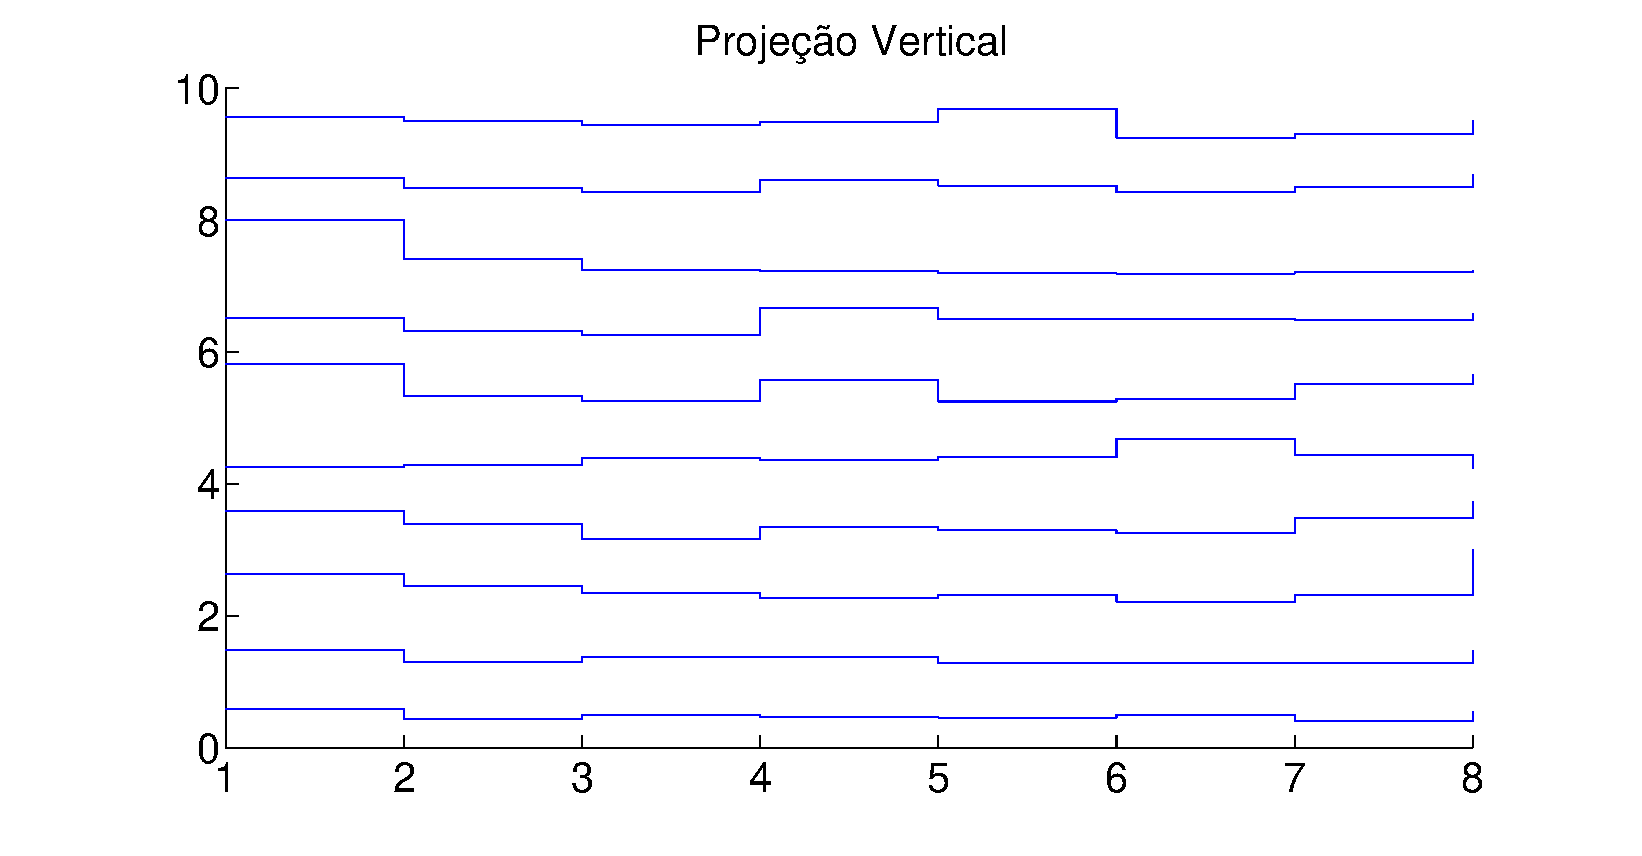
\includegraphics[height=5cm]{imagens/projecaoVertical.eps}
\caption{Projeção vertical.}
\label{fig:pv}
\end{figure}

\subsubsection{Posição e valor de pico maximo horizontal e vertical}
A posição e valor do pico máximo é utilizado para obter uma informação quanto a
forma do caractere. Abaixo temos os valores médios encontrados dentro da base da
dados.

\begin{table}[h]
\centering
\begin{tabular}{|c|c|c|c|c|}
\hline
          & \multicolumn{2}{c|}{Pico projeção vertical} & \multicolumn{2}{c|}{Pico projeção horizontal} \\ \hline
Caractere & Média             & Desvio padrão           & Média              & Desvio padrão            \\ \hline
0         & 0.0371            & 0.0412                  & 0.1723             & 0.0546                   \\ \hline
1         & 0.0527            & 0.0545                  & 0.1397             & 0.0364                   \\ \hline
2         & 0.1258            & 0.0068                  & 0.1607             & 0.0339                   \\ \hline
3         & 0.0843            & 0.0530                  & 0.1356             & 0.0098                   \\ \hline
4         & 0.0986            & 0.0066                  & 0.0669             & 0.0420                   \\ \hline
5         & 0.0160            & 0.0008                  & 0.0546             & 0.0099                   \\ \hline
6         & 0.0471            & 0.0213                  & 0.0931             & 0.0109                   \\ \hline
7         & 0.0162            & 0.0007                  & 0.0611             & 0.0265                   \\ \hline
8         & 0.0586            & 0.0489                  & 0.1306             & 0.0532                   \\ \hline
9         & 0.0620            & 0.0317                  & 0.1306             & 0.0532                   \\ \hline
\end{tabular}
\caption{Localização média dos picos de máximos dos caracteres em cada
projeção.}
\end{table}

\begin{table}[h]
\centering
\begin{tabular}{|c|c|c|c|c|}
\hline
          & \multicolumn{2}{c|}{Pico projeção vertical} & \multicolumn{2}{c|}{Pico projeção horizontal} \\ \hline
Caractere & Média             & Desvio padrão           & Média              & Desvio padrão            \\ \hline
0         & 0.1358            & 0.0456                  & 0.1074             & 0.0131                   \\ \hline
1         & 0.1657            & 0.1156                  & 0.1263             & 0.0055                   \\ \hline
2         & 0.1888            & 0.0323                  & 0.0807             & 0.0125                   \\ \hline
3         & 0.1464            & 0.0427                  & 0.1000             & 0.0087                   \\ \hline
4         & 0.1400            & 0.0423                  & 0.1228             & 0.0113                   \\ \hline
5         & 0.1571            & 0.0349                  & 0.0916             & 0.0137                   \\ \hline
6         & 0.1296            & 0.0142                  & 0.1002             & 0.0224                   \\ \hline
7         & 0.1973            & 0.0306                  & 0.0727             & 0.0270                   \\ \hline
8         & 0.1449            & 0.0209                  & 0.1199             & 0.0096                   \\ \hline
9         & 0.1315            & 0.0142                  & 0.1017             & 0.0210                   \\ \hline
\end{tabular}
\caption{Valor médio dos picos de máximos dos caracteres em cada projeção.}
\end{table}





\section{O algoritmo de vizinhos mais próximos}

O algoritmo de vizinho mais próximo foi proposto por Cover e Hart em 1966. Essa técnica é um método de estimação de densidade bastante simples conceitualmente e de fácil implementação.

K vizinhos mais próximos é um algoritmo simples que armazena todos os casos disponíveis e classifica novos casos com base em uma medida de similaridade (funções de distância). KNN foi usado na estimativa estatística e reconhecimento de padrões já o início da década de 1970, como uma técnica não-paramétrica.

Um caso é classificado pelo voto da maioria de seus vizinhos, com o caso sendo atribuído à classe mais comum entre os seus K vizinhos mais próximos medidos por um função de distância. Se K = 1, então o processo é simplesmente atribuído à classe de seu vizinho mais próximo.

O Pseudocódigo é definido como uma listagem de etapas sequenciais para resolver um problema computacional. Pseudocódigo é utilizado por programadores de computador para traduzir mentalmente cada passo computacional em um conjunto de instruções de programação envolvendo várias operações matemáticas (adição, subtração, funções multiplicação, divisão, potência e transcendentais, diferenciação / integração, etc.) e recursos (vetores, matrizes, gráficos, de entrada / saída, etc), a fim de resolver um problemas analíticos. Segue uma listagem de pseudocódigo para o método de classificação k-vizinho mais próximo utilizando validação cruzada. \\
\\
Inicializa o $n \times n$ distância matriz $\textbf{D}$ \\
Inicializa o $\Omega \times \Omega$ matriz confusão $\textbf{C}$ \\

set $t \leftarrow 0$, $TotAcc \leftarrow 0$, e define $NumIterations$ equivalente ao número desejado de  iterações (re-partições). 
 
Calcular distâncias entre todas as amostras de entrada e armazenar em $n \times n$ matriz $\textbf{D} $. ((Para um grande número de amostras, usar apenas o menor ou triangular superior de $\textbf{D}$ para armazenamento, uma vez que é uma simétrica quadrada matriz).

Para $t \leftarrow 1$ até $NumIterations$ faz set $\textbf{C} \leftarrow 0$, e $n_{total} \leftarrow 0$, particionar as amostras de entrada em $\kappa$ grupos de tamanho igual.
Para $fold \leftarrow 1$ até $\kappa$ atribuir amostras no $foldth$ partição para testar e usar as amostras restantes para o treinamento. Definir o número de amostras usado para testes quanto  $n_{test}$.\\

set $n_{total} \leftarrow n_{total}+n_{test}$\\

Para $i \leftarrow 1$ to $n_{test}$\ fazer por amostra de teste $\textbf{x}_i$ determinar a
$k$ próximas amostras de treinamento com base nas distâncias. determinar $\hat{\omega}$ ,o rótulo de classe mais freqüente entre os $k$ mais próximo amostras de treinamento. Incrementar matriz de confusão $\textbf{C}$ por um elemento em $c_{\omega,\hat{\omega}}$ , onde $\omega$ é o verdadeiro $\hat{\omega}$ o rótulo de classe previsto para amostra de teste $\textbf{x}_i$ . Se $\omega =\hat{\omega}$ em seguida, o incremento de um ocorrerá na diagonal da matriz de confusão, de outro modo, o incremento irá ocorrer em um off-diagonal.
Determinar a precisão da classificação usando $Acc = \frac{\sum_j^{\Omega}c_{jj}}{n_{total}}$ onde $c_{jj}$  é o elemento diagonal da matriz confusão $\textbf{C}$, calcular $TotAcc = TotAcc + Acc$, calcular $AvgAcc = TotAcc/NumIterations$

%%%%%%%%%%%%%%%%%%%%%%%%%%%%%%%%%%%%%%%%%%%%%%%%%%%%%%%%%%%%%%%%%%%%%%%%%%%%%%%%
\section{ALGORITMO PROPOSTO}

%%%%%%%%%%%%%%%%%%%%%%%%%%%%%%%%%%%%%%%%%%%%%%%%%%%%%%%%%%%%%%%%%%%%%%%%%%%%%%%%
\subsection{Força Bruta de Busca kNN}

%%%%%%%%%%%%%%%%%%%%%%%%%%%%%%%%%%%%%%%%%%%%%%%%%%%%%%%%%%%%%%%%%%%%%%%%%%%%%%%%
\subsubsection{Princípio}

Seja R = $\{r_1; r_2; \cdots ; r_m\}$ um conjunto de pontos de referência m com valores em $\Re^d$, e deixe Q = $\{q_1; q_2; \cdots ; q_m\}$ um conjunto de pontos de n consulta no mesmo espaço. O problema de pesquisa kNN consiste em procurar os k vizinhos mais próximos de cada ponto de consulta $q_i$ $\in$ Q na referência fixado R dada uma determinada distância. Geralmente, a distância euclidiana ou a Manhattan é usado, mas qualquer outra distância pode ser utilizado em substituição, tais como a norma Chebyshov ou a distância de Mahalanobis. A Figura \ref{fig:Figura03} ilustra o problema kNN com k = 3, bem como um conjunto de pontos com valores de $\Re^2$.

\begin{figure}[H]
\centering

\includegraphics[height=5cm]{KNN.png}

\caption{Ilustração do problema de pesquisa kNN em $\Re^2$ com k = 3, utilizando a distância euclidiana.}
\label{fig:Figura03}
\end{figure}

Uma maneira de procurar o kNN é o algoritmo de "força bruta" (BF observado) também chamado de "pesquisa exaustiva". Para cada ponto de consulta $q_i$, o algoritmo BF tem o seguintes passos:\\

1. Calcule todas as distâncias entre $q_i$ e $r_j$, j $\in$ [1, m].\\

2. Organize as distâncias computadas.\\

3. Selecione os pontos de referência k correspondentes aos k menores distâncias.\\

4. Repita os passos 1 a 3. para todos os pontos da consulta.\\

A questão principal deste algoritmo é a sua enorme complexidade: O (nmd) para as distâncias nm computadorizada (aproximadamente 2nmd adições / subtrações e multiplicações NMD) e
O (nmlogm) para os tipos de n realizados (número de comparações dizer).

Vários algoritmos KNN têm sido propostos a fim de reduzir o tempo de computação. De um modo geral, a ideia consiste em reduzir o número de distâncias calculado [15]. Por exemplo, alguns algoritmos [14] particiona os conjuntos de pontos, utilizando uma estrutura $k_d$-árvore, e só calcular distâncias dentro volumes próximos. De acordo com as nossas experiências, a utilização de um tal método é geralmente mais rápido do que um método CPU-Based BF até o fator 10.\\

%%%%%%%%%%%%%%%%%%%%%%%%%%%%%%%%%%%%%%%%%%%%%%%%%%%%%%%%%%%%%%%%%%%%%%%%%%%%%%%%
\subsubsection{Algoritmo de Ordenação}

O segundo passo do algoritmo BF é o tipo de as distâncias computadas. Nesta seção, vamos discutir a escolha do algoritmo de classificação.

O Quicksort é um algoritmo popular que na prática, é um dos algoritmos mais rápidos. No entanto, é recursivo e CUDA não permite funções recursivas. Como consequência, não pode ser usado nessa execução. A complexidade é O(n log n), tanto nos piores e médios casos. É também um dos algoritmos mais rápidos e simples de implementar.

No entanto, tendo em mente que estamos interessados apenas nas menores k elementos, sendo k geralmente muito pequeno comparado a $N_P$ e $N_Q$, considerou-se usando uma variante tipo de inserção que só produz os menores elementos k.\\ 

%%%%%%%%%%%%%%%%%%%%%%%%%%%%%%%%%%%%%%%%%%%%%%%%%%%%%%%%%%%%%%%%%%%%%%%%%%%%%%%%
\subsubsection{Implementação CUDA}

O método BF é, por natureza altamente paralelizável. Esta propriedade faz com que o método BF seja perfeitamente adequado para a implementação GPU. O método BF tem duas etapas: a computação distância e da classificação. Para simplificar, supõe que a referência e consulta, ambos contêm n pontos. 

O cálculo das distâncias $n^2$ podem ser totalmente paralelizado uma vez que as distâncias entre os pares de pontos são independentes. Dois tipos de memória são utilizados: memória global e memória de textura. A memória global tem uma enorme largura de banda, mas as performances diminuem se os acessos de memória são não-aglutinados. Em tal caso, a memória de textura é uma boa opção porque há menos penalidades para leituras não-aglutinados. Como conseqüência, foi utilizado memória global para armazenar o conjunto de consulta (leituras unidas), e memória de textura para o conjunto de referência (leituras não se uniram). Assim, obtém-se um melhor desempenho do que quando se utiliza a memória global e memória compartilhada como proposto no exemplo multiplicação de matrizes fornecidas no SDK CUDA. 

As n ordenações também podem ser paralelizadas enquanto as operações realizadas durante um determinada triagem de n valores não são claramente independentes um do outro. Cada segmento classifica todas as distâncias calculadas para um determinado ponto de consulta. A triagem consiste em comparar e trocar muitas distâncias em uma ordem não-previsível. Portanto, os acessos de memória não são aglutinadas, indicando que a memória de textura pode ser apropriado. No entanto, é uma memória só de leitura. Apenas a memória global permite leituras e escritas. Isso penaliza o desempenho de classificação.

%%%%%%%%%%%%%%%%%%%%%%%%%%%%%%%%%%%%%%%%%%%%%%%%%%%%%%%%%%%%%%%%%%%%%%%%%%%%%%%%
\section{RESULTADOS OBTIDOS}

%%%%%%%%%%%%%%%%%%%%%%%%%%%%%%%%%%%%%%%%%%%%%%%%%%%%%%%%%%%%%%%%%%%%%%%%%%%%%%%%
\section*{CONCLUSÃO}
%%%%%%%%%%% COLOCAR TEXTO %%%%%%%%%%%%%%%%



%%%%%%%%%%%%%%%%%%%%%%%%%%%%%%%%%%%%%%%%%%%%%%%%%%%%%%%%%%%%%%%%%%%%%%%%%%%%%%%%
%%%%%%%%    Bibliografia  %%%%%%%%
\begin{thebibliography}{1}

\bibitem{IEEEhowto:kopka}
HERBERT SCHANTZ (1982), The History of OCR. Manchester Center, VT: Recognition Technologies Users Association.

\bibitem{IEEEhowto:kopka}
THE MNIST DATABASE, http://yann.lecun.com/exdb/mnist/ An introduction to neural computing. Aleksander, I. and Morton, H. 2nd edition.

\bibitem{IEEEhowto:kopka}
Deolinda M. P. Aguieiras de Lima, http://mesonpi.cat.cbpf.br/naj/redesneurais.pdf/

\bibitem{IEEEhowto:kopka}
JEFF HEATON, Introduction to Neural Networks with Java, second edition.

\bibitem{IEEEhowto:kopka}
Facon, Jacques; Morfologia Matemática: Teoria e Exemplos. Curitiba,
 Brasil, 1996

\bibitem{IEEEhowto:kopka}
 Alessandra Bussador; Localização Automática de Placas de Veículos em Fotos
Digitais Utilizando Abordagem Granulométrica. Curitiba,
 Brasil, 1996

\bibitem{IEEEhowto:kopka}
GONZALEZ, Rafael C.; WOODS, Richard E. Processamento de Imagens Digitais. 1. ed. São Paulo: Edgard Blücher, 2000.

\bibitem{IEEEhowto:kopka}
PARKER, J. R.. Algorithms for Image Processing and Computer Vision. New York, John wiley $ \& $ Sons, 1997. 

\bibitem{IEEEhowto:kopka}
RUSS, John C. . The image processing handbook. 2 ed., Boca Raton, CRC Press, 1995.

\bibitem{IEEEhowto:kopka}
MARQUES FILHO, Ogê $ \& $ VIEIRA NETO, Hugo. Processamento digital de Imagens. Rio de Janeiro, Brasport, 1999.

\bibitem{IEEEhowto:kopka}
QUEIROZ, J. E. R.; GOMES, H. M. Introdução ao Processamento Digital de Imagens. 2001. 

\bibitem{IEEEhowto:kopka}
GOMES, J.; VELHO, L. Image Processing for Computer Graphics. Springer-Verlag, 1997. 

\bibitem{IEEEhowto:kopka}
REBOUÇAS FILHO, P. P.Notas de Aula da Disciplina Processamento Digital de Imagens. 2014. 

\bibitem{IEEEhowto:kopka}
S. Arya, D. M. Mount, N. S. Netanyahu, R. Silverman, and A. Y. Wu. An optimal algorithm for approximate nearest neighbor searching fixed dimensions. Journal of the ACM, 45(6):891–923, 1998.

\bibitem{IEEEhowto:kopka}
Q. Lv,W. Josephson, Z.Wang, M. Charikar, and K. Li. Multiprobe lsh: efficient indexing for high-dimensional similarity search. In VLDB ’07: Proceedings of the 33rd international conference on Very large data bases, pages 950–961. VLDB Endowment, 2007.

\end{thebibliography}


\end{document}
